

%% AAPT Physics Olympiad F=ma Questions
%%----------------------------------------


%% this section contains 23 problems


%% PhysicsOlympiad 2015
%%----------------------------------------
\element{aapt}{ %% Olympiad-A2
\begin{question}{Olympiad-2015-Q01}
    A \SI{600}{\meter} wide river flows directly south at \SI{4.0}{\meter\per\second}.
    A small motor boat travels at \SI{5.0}{\meter\per\second} in still water and points in such a direction so that it will travel directly east relative to the land.
    \begin{center}
    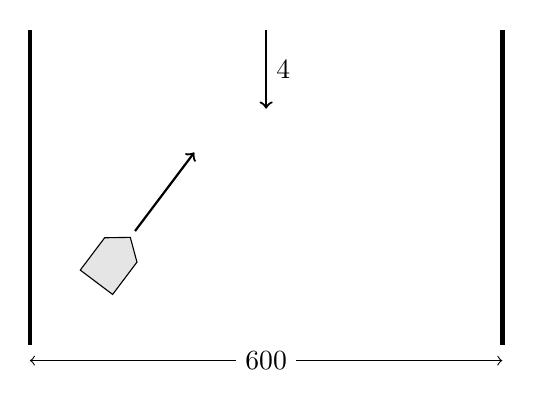
\begin{tikzpicture}
        %% Banks
        \draw[ultra thick] (-3,-2) -- (-3,2);
        \draw[ultra thick] (+3,-2) -- (+3,2);
        \draw[<->] (-3,-2.2) -- (+3,-2.2) node[pos=0.5,anchor=center,fill=white] {\SI{600}{\meter}};
        %% Boat
        \node[rotate=53,minimum size=0.5cm] (B) at (-2,-1) {};
        \draw[fill=white!90!black] (B.east) ++ (53:0.20) -- (B.south east) -- (B.south west) -- (B.north west) -- (B.north east) --cycle;
        \draw[thick,->] (B.east) ++(53:0.3) -- ++(53:1.25);
        %% Current
        \draw[thick,->] (0,+2) -- (0,+1) node[pos=0.5,anchor=west] {\SI{4}{\meter\per\second}};
    \end{tikzpicture}
    \end{center}
    The time it takes to cross the river is closest to:
    \begin{multicols}{3}
    \begin{choices}
        \wrongchoice{\SI{67}{\second}}
        \wrongchoice{\SI{120}{\second}}
        \wrongchoice{\SI{150}{\second}}
      \correctchoice{\SI{200}{\second}}
        \wrongchoice{\SI{600}{\second}}
    \end{choices}
    \end{multicols}
\end{question}
}

\element{aapt}{ %% Olympiad-A2
\begin{question}{Olympiad-2015-Q21}
    An object launched vertically upward from the ground with a speed of \SI{50}{\meter\per\second} bounces off of the ground on the return trip with a coefficient of restitution given by $C_R=0.9$,
        meaning that immediately after a bounce the upward speed is \SI{90}{\percent} of the previous downward speed.
    The ball continues to bounce like this;
        what is the total amount of time between when the ball is launched and when it finally comes to a rest?
    Assume the collision time is zero; the bounce is instantaneous.
    Treat the problem as ideally classical and ignore any quantum effects that might happen for very small bounces.
    \begin{multicols}{2}
    \begin{choices}
        \wrongchoice{\SI{71}{\second}}
      \correctchoice{\SI{100}{\second}}
        \wrongchoice{\SI{141}{\second}}
        \wrongchoice{\SI{1000}{\second}}
        \wrongchoice{$\infty$ (the ball never comes to a rest)}
    \end{choices}
    \end{multicols}
\end{question}
}


%% PhysicsOlympiad 2014
%%----------------------------------------


%% PhysicsOlympiad 2013
%%----------------------------------------
\element{aapt}{ %% Olympiad-A2
\begin{question}{Olympiad-2013-Q03}
    Tom throws a football to Wes, who is a distance $l$ away.
    Tom can control the time of flight $t$ of the ball by choosing any speed up to $v_{max}$
        and any launch angle between \ang{0} and \ang{90}.
    Ignore air resistance and assume Tom and Wes are at the same height.
    Which of the following statements is \emph{incorrect}?
    \begin{choices}
        %% remember R = \frac{v^2}{g}\sin 2\theta
        \wrongchoice{If $v_{max}<\sqrt{gl}$, the ball cannot reach Wes at all.}
        \wrongchoice{Assuming the ball can reach Wes, as $v_{max}$ increases with $l$ held fixed, the minimum value of $t$ decreases.}
        \wrongchoice{Assuming the ball can reach Wes, as $v_{max}$ increases with $l$ held fixed, the maximum value of $t$ increases.}
        \wrongchoice{Assuming the ball can reach Wes, as $l$ increases with $v_{max}$ held fixed, the minimum value of $t$ increases.}
      \correctchoice{Assuming the ball can reach Wes, as $l$ increases with $v_{max}$ held fixed, the maximum value of $t$ increases.}
    \end{choices}
\end{question}
}


%% PhysicsOlympiad 2012
%%----------------------------------------
\element{aapt}{ %% Olympiad-A2
\begin{question}{Olympiad-2012-Q02}
    A cannonball is launched with initial velocity of magnitude $v_0$
        over a horizontal surface.
    At what minimum angle $\theta_{min}$ above the horizontal should the
        cannonball be launched so that it rises to a height $H$
        which is larger than the horizontal distance $R$ that it will
        travel when it returns to the ground?
    \begin{choices}
      \correctchoice{$\theta_{min}=\ang{76}$}
        \wrongchoice{$\theta_{min}=\ang{72}$}
        \wrongchoice{$\theta_{min}=\ang{60}$}
        \wrongchoice{$\theta_{min}=\ang{45}$}
        \wrongchoice{There is no such angle, as $R>H$ for all range problems.}
    \end{choices}
\end{question}
}

\element{aapt}{ %% Olympiad-A2
\begin{question}{Olympiad-2012-Q06}
    Two cannons are arranged vertically, with the lower cannon pointing upward
        (towards the upper cannon) and the upper cannon pointing downward
        (towards the lower cannon), \SI{200}{\meter\per\second} above the lower cannon.
    Simultaneously, they both fire.
    The muzzle velocity of the lower cannon is \SI{25}{\meter\per\second}
        and the muzzle velocity of the upper cannon is \SI{55}{\meter\per\second}.
    \begin{center}
        \includegraphics[keepaspectratio,scale=0.8]{Olympiad2012-Q06}
    \end{center}
    How long after the cannons fire do the projectiles collide?
    \begin{multicols}{3}
    \begin{choices}
        \wrongchoice{\SI{2.2}{\second}}
      \correctchoice{\SI{2.5}{\second}}
        \wrongchoice{\SI{3.6}{\second}}
        \wrongchoice{\SI{6.7}{\second}}
        \wrongchoice{\SI{8.0}{\second}}
    \end{choices}
    \end{multicols}
\end{question}
}

\element{aapt}{ %% Olympiad-A2
\begin{question}{Olympiad-2012-Q07}
    Two cannons are arranged vertically, with the lower cannon pointing upward
        (towards the upper cannon) and the upper cannon pointing downward
        (towards the lower cannon), \SI{200}{\meter\per\second} above the lower cannon.
    Simultaneously, they both fire.
    The muzzle velocity of the lower cannon is \SI{25}{\meter\per\second}
        and the muzzle velocity of the upper cannon is \SI{55}{\meter\per\second}.
    \begin{center}
        \includegraphics[keepaspectratio,scale=0.8]{Olympiad2012-Q06}
    \end{center}
    How far beneath the top cannon do the projectiles collide?
    \begin{multicols}{3}
    \begin{choices}
        \wrongchoice{\SI{31}{\meter}}
        \wrongchoice{\SI{67}{\meter}}
        \wrongchoice{\SI{110}{\meter}}
        \wrongchoice{\SI{140}{\meter}}
      \correctchoice{\SI{170}{\meter}}
    \end{choices}
    \end{multicols}
\end{question}
}


%% PhysicsOlympiad 2011
%%----------------------------------------
\element{aapt}{ %% Olympiad-A2
\begin{question}{Olympiad-2011-Q05}
    A crude approximation is that the Earth travels in a circular orbit
        about the Sun at constant speed, at a distance of \SI{150 000 000}{\kilo\meter}
        from the Sun.
    Which of the following is the closest for the acceleration of the Earth in this orbit?
    \begin{multicols}{2}
    \begin{choices}
        %% a = v^2 / r = ( (2\pi r)/t )^2 / r = 4\pi^2 r / t^2
        \wrongchoice{exactly \SI{0}{\meter\per\second\squared}}
      \correctchoice{\SI{0.006}{\meter\per\second\squared}}
        \wrongchoice{\SI{0.6}{\meter\per\second\squared}}
        \wrongchoice{\SI{6}{\meter\per\second\squared}}
        \wrongchoice{\SI{10}{\meter\per\second\squared}}
    \end{choices}
    \end{multicols}
\end{question}
}


%% PhysicsOlympiad 2010
%%----------------------------------------
\element{aapt}{ %% Olympiad-A2
\begin{question}{Olympiad-2010-Q04}
    Two teams of movers are lowering a piano from the window
        of a \num{10} floor apartment building.
    The rope breaks when the piano is \SI{30}{\meter} above the ground.
    The movers on the ground, alerted by the shouts of the movers above,
        first notice the piano when it is \SI{14}{\meter} above the ground.
    How long do they have to get out of the way before the piano hits the ground?
    \begin{multicols}{3}
    \begin{choices}
      \correctchoice{\SI{0.66}{\second}}
        \wrongchoice{\SI{0.78}{\second}}
        \wrongchoice{\SI{1.67}{\second}}
        \wrongchoice{\SI{1.79}{\second}}
        \wrongchoice{\SI{2.45}{\second}}
    \end{choices}
    \end{multicols}
\end{question}
}

\element{aapt}{ %% Olympiad-A2
\begin{question}{Olympiad-2010-Q05}
    Two projectiles are launched from a 35 meter ledge as shown in the diagram.
    One is launched from a 37 degree angle above the horizontal and the
        other is launched from 37 degrees below the horizontal.
    Both of the launches are given the same initial speed of $v_0=\SI{50}{\meter\per\second}$.
    \begin{center}
    \begin{tikzpicture}
        %% Surface
        \draw[thick] (-1.2,0) -- (0,0) -- (0,-3) -- (5,-3);
        \draw[dashed] (0,0) -- (0.5,0);
        %% Labels
        \draw[<->] (-1,0) -- (-1,-3) node[pos=0.5,anchor=center,fill=white] {\SI{35}{\meter}};
        %% Trajectories
        \draw[dashed,domain=0:11.8,samples=20] plot ({0.342*\x}, {0.257*\x-0.0429*\x*\x});
        \draw[dashed,domain=0:5.9,samples=20] plot ({0.342*\x}, {-0.257*\x-0.0429*\x*\x});
    \end{tikzpicture}
    \end{center}
    The difference in the times of flight for these two projectiles,
        $t_1-t_2$, is closest to
    \begin{multicols}{3}
    \begin{choices}
        \wrongchoice{\SI{3}{\second}}
        \wrongchoice{\SI{5}{\second}}
      \correctchoice{\SI{6}{\second}}
        \wrongchoice{\SI{8}{\second}}
        \wrongchoice{\SI{10}{\second}}
    \end{choices}
    \end{multicols}
\end{question}
}

\element{aapt}{ %% Olympiad-A2
\begin{question}{Olympiad-2010-Q06}
    A projectile is launched across flat ground at an angle $\theta$ to the
        horizontal and travels in the absence of air resistance.
    It rises to a maximum height $H$ and lands a horizontal distance $R$ away.
    What is the ratio $\frac{H}{R}$?
    \begin{multicols}{2}
    \begin{choices}
        \wrongchoice{$\tan\theta$}
        \wrongchoice{$2\tan\theta$}
        \wrongchoice{$\dfrac{2}{\tan\theta}$}
        \wrongchoice{$\dfrac{1}{2}\tan\theta$}
      \correctchoice{$\dfrac{1}{4}\tan\theta$}
    \end{choices}
    \end{multicols}
\end{question}
}


%% PhysicsOlympiad 2009
%%----------------------------------------
\element{aapt}{ %% Olympiad-A2
\begin{question}{Olympiad-2009-Q06}
    An object is thrown with a fixed initial speed $v_0$ at various
        angles $\alpha$ relative to the horizon.
    At some constant height $h$ above the launch point the speed $v$
        of the object is measured as a function of the initial angle $\alpha$.
    Which of the following best describes the dependence of $v$ on $\alpha$?
        (Assume that the height $h$ is achieved, and assume that there is no air resistance.)
    \begin{choices}
        \wrongchoice{$v$ will increase monotonically with $\alpha$.}
        \wrongchoice{$v$ will increase to some critical value $v_{max}$ and then decrease.}
      \correctchoice{$v$ will remain constant, independent of $\alpha$.}
        \wrongchoice{$v$ will decrease to some critical value $v_{min}$ and then increase.}
        \wrongchoice{None of the provided.}
    \end{choices}
\end{question}
}

\element{aapt}{ %% Olympiad-A2
\begin{question}{Olympiad-2009-Q10}
    A person standing on the edge of a fire escape simultaneously launches two apples,
        one straight up with a speed of \SI{7}{\meter\per\second}
        and the other straight down at the same speed.
    How far apart are the two apples 2 seconds after they were thrown,
        assuming that neither has hit the ground?
    \begin{multicols}{2}
    \begin{choices}
        \wrongchoice{\SI{14}{\meter}}
        \wrongchoice{\SI{20}{\meter}}
      \correctchoice{\SI{28}{\meter}}
        \wrongchoice{\SI{34}{\meter}}
        \wrongchoice{\SI{56}{\meter}}
    \end{choices}
    \end{multicols}
\end{question}
}

\element{aapt}{ %% Olympiad-A2
\begin{question}{Olympiad-2009-Q19}
    A certain football quarterback can throw a football a maximum range
        of \num{80} meters on level ground.
    What is the highest point reached by the football if thrown this maximum range?
    Ignore air friction.
    \begin{multicols}{3}
    \begin{choices}
        \wrongchoice{\SI{10}{\meter}}
      \correctchoice{\SI{20}{\meter}}
        \wrongchoice{\SI{30}{\meter}}
        \wrongchoice{\SI{40}{\meter}}
        \wrongchoice{\SI{50}{\meter}}
    \end{choices}
    \end{multicols}
\end{question}
}


%% PhysicsOlympiad 2008
%%----------------------------------------
\element{aapt}{ %% Olympiad-A2
\begin{question}{Olympiad-2008-Q06}
    A cannon fires projectiles on a flat range at a
        fixed speed but with variable angle.
    The maximum range of the cannon is $L$.
    What is the range of the cannon when it fires at an angle
        $\frac{\pi}{6}$ above the horizontal?
    Ignore air resistance.
    \begin{multicols}{3}
    \begin{choices}
      \correctchoice{$\dfrac{\sqrt{3}}{2}L$}
        \wrongchoice{$\dfrac{1}{\sqrt{2}}L$}
        \wrongchoice{$\dfrac{1}{\sqrt{3}}L$}
        \wrongchoice{$\dfrac{1}{2}L$}
        \wrongchoice{$\dfrac{1}{3}L$}
    \end{choices}
    \end{multicols}
\end{question}
}


%% PhysicsOlympiad 2007
%%----------------------------------------
\element{aapt}{ %% Olympiad-A2
\begin{question}{Olympiad-2007-Q17}
    A small point-like object is thrown horizontally off of a
        \SI{50.0}{\meter} high building with an initial speed
        of \SI{10.0}{\meter\per\second}.
    At any point along the trajectory there is an acceleration
        component tangential to the trajectory and an acceleration
        component perpendicular to the trajectory.
    How many seconds after the object is thrown is the tangential
        component of the acceleration of the object equal to twice
        the perpendicular component of the acceleration of the object?
    Ignore air resistance.
    \begin{multicols}{2}
    \begin{choices}
      \correctchoice{\SI{2.00}{\second}}
        \wrongchoice{\SI{1.50}{\second}}
        \wrongchoice{\SI{1.00}{\second}}
        \wrongchoice{\SI{0.50}{\second}}
        \wrongchoice{The building is not high enough for this to occur.}
    \end{choices}
    \end{multicols}
\end{question}
}


%% PhysicsOlympiad 2004
%%----------------------------------------
\element{aapt}{ %% Olympiad-A2
\begin{question}{Olympiad-2004-Q04}
    A hunter in a forest walks \SI{800}{\meter} west.
    He then turns south and walks \SI{400}{\meter} before turning west again and walking a final \SI{300}{\meter}.
    At the end of the walk,
        what is the magnitude of the hunter's displacement from the beginning?
    \begin{multicols}{3}
    \begin{choices}
        \wrongchoice{\SI{640}{\meter}}
        \wrongchoice{\SI{890}{\meter}}
      \correctchoice{\SI{1170}{\meter}}
        \wrongchoice{\SI{1390}{\meter}}
        \wrongchoice{\SI{1500}{\meter}}
    \end{choices}
    \end{multicols}
\end{question}
}

\element{aapt}{ %% Olympiad-A2
\begin{question}{Olympiad-2004-Q05}
    Robin Hood aims his longbow horizontally at a target's bull eye \SI{30}{\meter} away.
    If the arrow strikes the target exactly \SI{1.0}{\meter} below the bull's eye,
        how fast did the arrow move as it was shot from the bow?
    Assume air resistance is negligible.
    \begin{multicols}{3}
    \begin{choices}
        \wrongchoice{\SI{6.0}{\meter\per\second}}
        \wrongchoice{\SI{13}{\meter\per\second}}
        \wrongchoice{\SI{33}{\meter\per\second}}
      \correctchoice{\SI{67}{\meter\per\second}}
        \wrongchoice{\SI{150}{\meter\per\second}}
    \end{choices}
    \end{multicols}
\end{question}
}


%% PhysicsOlympiad 2003
%%----------------------------------------


%% PhysicsOlympiad 1998
%%----------------------------------------
\element{aapt}{ %% Olympiad-A2
\begin{question}{olympiad-1998-q03}
    In a rescue attempt, a hovering helicopter drops a life preserver to a swimmer being swept downstream by a river current of constant velocity $v$.
    The helicopter is at a height of \SI{9.8}{\meter}.
    The swimmer is \SI{6.0}{\meter} upstream from a point directly under the helicopter when the life preserver is released.
    It lands \SI{2.0}{\meter} in front of the swimmer.
    How fast is the current flowing?
    Neglect air resistance.
    \begin{multicols}{3}
    \begin{choices}
        \wrongchoice{\SI{13.7}{\meter\per\second}}
        \wrongchoice{\SI{9.8}{\meter\per\second}}
        \wrongchoice{\SI{6.3}{\meter\per\second}}
      \correctchoice{\SI{2.8}{\meter\per\second}}
        \wrongchoice{\SI{2.4}{\meter\per\second}}
    \end{choices}
    \end{multicols}
\end{question}
}


%% PhysicsOlympiad 1997
%%----------------------------------------
\element{aapt}{ %% Olympiad-A2
\begin{question}{olympiad-1997-q02}
    A flare is dropped from a plane flying over level ground at a velocity of \SI{70}{\meter\per\second} in the horizontal direction.
    At the instant the flare is released, the plane begins to accelerate horizontally at \SI{0.75}{\meter\per\second\squared}.
    The flare takes \SI{4.0}{\second} to reach the ground.
    Assume air resistance is negligible.
    Relative to a spot directly under the flare at release,
        the flare lands directly on the spot.
    \begin{choices}
        \wrongchoice{directly on the spot}
        \wrongchoice{\SI{6.0}{\meter} in front of the spot.}
        \wrongchoice{\SI{274}{\meter} in front of the spot.}
      \correctchoice{\SI{280}{\meter} in front of the spot.}
        \wrongchoice{\SI{286}{\meter} in front of the spot.}
    \end{choices}
\end{question}
}

\element{aapt}{ %% Olympiad-A2
\begin{question}{olympiad-1997-q03}
    A flare is dropped from a plane flying over level ground at a velocity of \SI{70}{\meter\per\second} in the horizontal direction.
    At the instant the flare is released, the plane begins to accelerate horizontally at \SI{0.75}{\meter\per\second\squared}.
    The flare takes \SI{4.0}{\second} to reach the ground.
    Assume air resistance is negligible.
    %% made independent
    %As seen by the pilot of the plane (in question \#2) and measured relative to a spot directly under the plane when the flare lands,
    As seen by the pilot of the plane and measured relative to a spot directly under the plane when the flare lands,
        the flare lands:
    \begin{choices}
        \wrongchoice{\SI{286}{\meter} behind the plane.}
      \correctchoice{\SI{6.0}{\meter} behind the plane.}
        \wrongchoice{directly under the plane.}
        \wrongchoice{\SI{12}{\meter} in front of the plane.}
        \wrongchoice{\SI{274}{\meter} in front of the plane}
    \end{choices}
\end{question}
}


%% PhysicsOlympiad 1996
%%----------------------------------------
\element{aapt}{ %% Olympiad-A2
\begin{question}{olympiad-1996-q02}
    A jogger runs with constant speed $v$ through a forest of pine trees.
    A pine cone starts to fall from a height $h$ when the jogger is directly below it.
    How far behind the jogger will the pine cone land?
    \begin{multicols}{3}
    \begin{choices}
      \correctchoice{$\sqrt{\dfrac{2hv^2}{g}}$}
        \wrongchoice{$\sqrt{\dfrac{hv^2}{g}}$}
        \wrongchoice{$\dfrac{gh^2}{2v^2}$}
        \wrongchoice{$\dfrac{2gh^2}{v^2}$}
        \wrongchoice{$\dfrac{v^2}{2g}$}
    \end{choices}
    \end{multicols}
\end{question}
}

\element{aapt}{ %% Olympiad-A2
\begin{question}{olympiad-1996-q04}
    A swimmer can swim with a velocity of \SI{1.0}{\meter\per\second} in still water.
    The swimmer wishes to swim directly across a river with a current of \SI{0.50}{\meter\per\second} directed from upstream to downstream.
    To end up directly across the river the swimmer must head at an angle of:
    \begin{choices}
        \wrongchoice{$\tan^{-1}\left(\dfrac{1}{2}\right)$ upstream.}
      \correctchoice{$\sin^{-1}\left(\dfrac{1}{2}\right)$ upstream.}
        \wrongchoice{directly across the river.}
        \wrongchoice{$\sin^{-1}\left(\dfrac{1}{2}\right)$ downstream}
        \wrongchoice{$\tan^{-1}\left(\dfrac{1}{2}\right)$ downstream}
    \end{choices}
\end{question}
}


%% PhysicsOlympiad 1995
%%----------------------------------------
\element{aapt}{ %% Olympiad-A2
\begin{question}{olympiad-1995-q02}
    A car is moving at a constant velocity to the right along a straight level highway.
    Just as the car passes a cliff,
        a rock falls straight down in the cliff’s reference system.
    Which of the accompanying curves best depicts the path the rock takes in the car's reference system?
    \begin{multicols}{3}
    \begin{choices}
        \AMCboxDimensions{down=-0.45cm}
        \wrongchoice{
            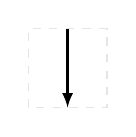
\begin{tikzpicture}
                \draw[dashed,white!90!black] (0,0) rectangle (1,1);
                \draw[thick,-latex] (0.5,1) -- (0.5,0);
            \end{tikzpicture}
        }
        \wrongchoice{
            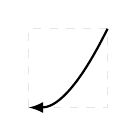
\begin{tikzpicture}
                \draw[dashed,white!90!black] (0,0) rectangle (1,1);
                %\draw[thick,-latex] (1,1) arc(0:-90:1);
                \draw[thick,-latex] (1,1) parabola bend (0,0) (0,0);
            \end{tikzpicture}
        }
        \wrongchoice{
            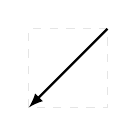
\begin{tikzpicture}
                \draw[dashed,white!90!black] (0,0) rectangle (1,1);
                \draw[thick,-latex] (1,1) -- (0,0);
            \end{tikzpicture}
        }
        %% ANS is E
        \correctchoice{
            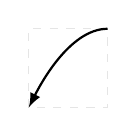
\begin{tikzpicture}
                \draw[dashed,white!90!black] (0,0) rectangle (1,1);
                %\draw[thick,-latex] (1,1) arc(90:180:1);
                \draw[thick,-latex] (1,1) parabola bend (1,1) (0,0);
            \end{tikzpicture}
        }
        \wrongchoice{
            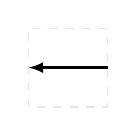
\begin{tikzpicture}
                \draw[dashed,white!90!black] (0,0) rectangle (1,1);
                \draw[thick,-latex] (1,0.5) -- (0,0.5);
            \end{tikzpicture}
        }
    \end{choices}
    \end{multicols}
\end{question}
}


%% PhysicsOlympiad 1994
%%----------------------------------------


\endinput


